
%*----------- SLIDE -------------------------------------------------------------
\begin{frame}[c]{Introdução}
    \transdissolve[duration=0.5]
    Linha de pesquisa focada em estudos e desenvolvimentos em \textbf{robótica submarina}, 
    aspectos de dinâmica computacional, aplicações de funções básicas de robótica e desenvolvimento de 
    tecnologias de busca e análise deste campo.
    \begin{figure}
        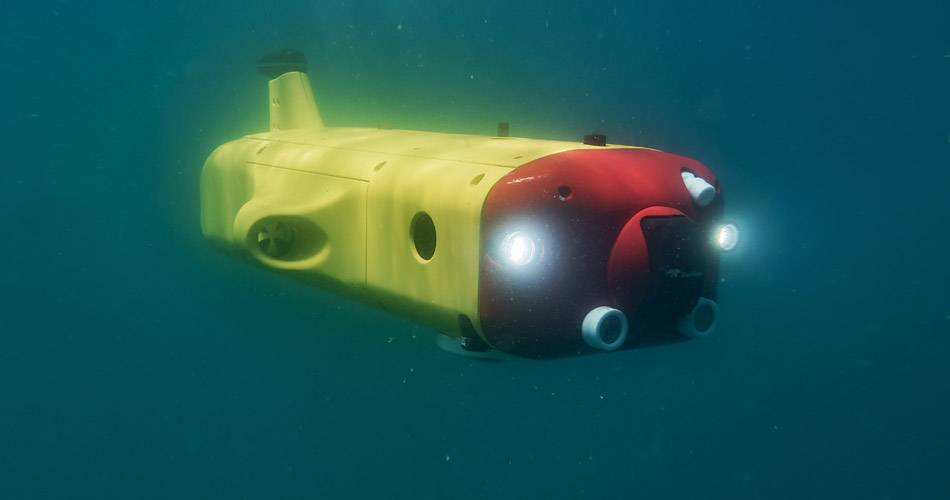
\includegraphics[height = 2.5cm, width=0.3\textwidth]{flatfish.jpg}
        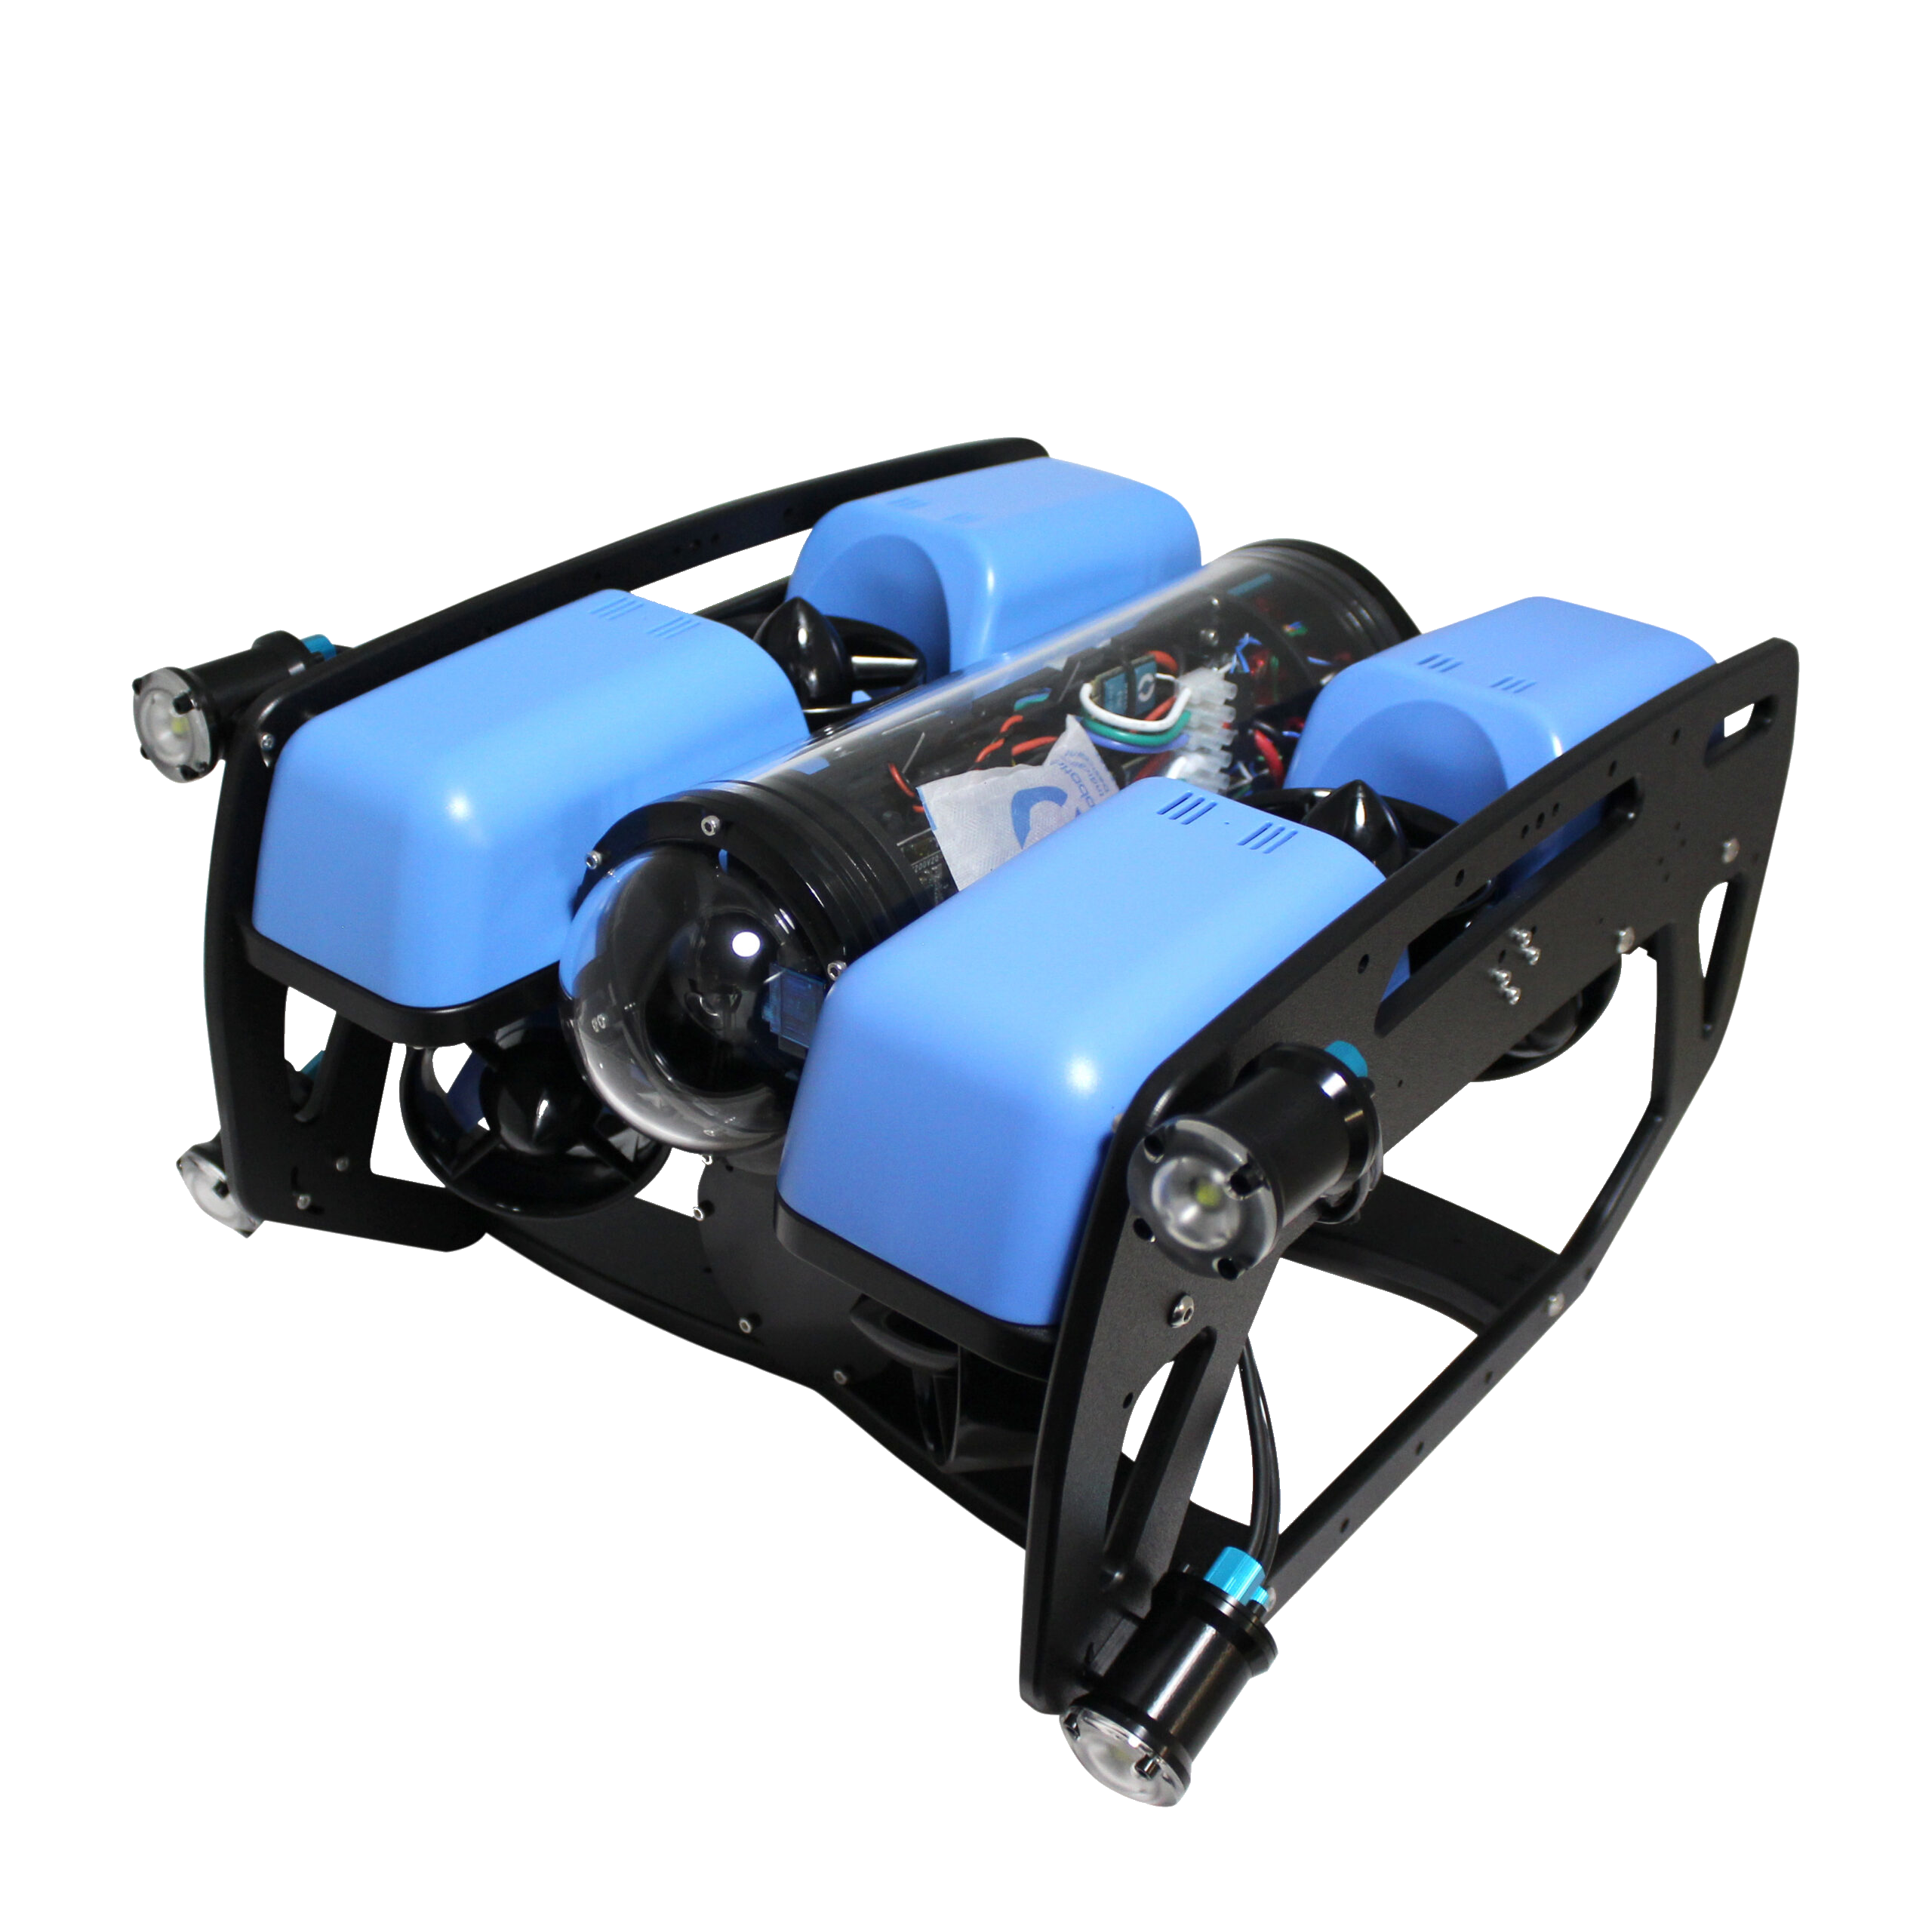
\includegraphics[height = 2.5cm, width=0.3\textwidth]{bluerov.png}
        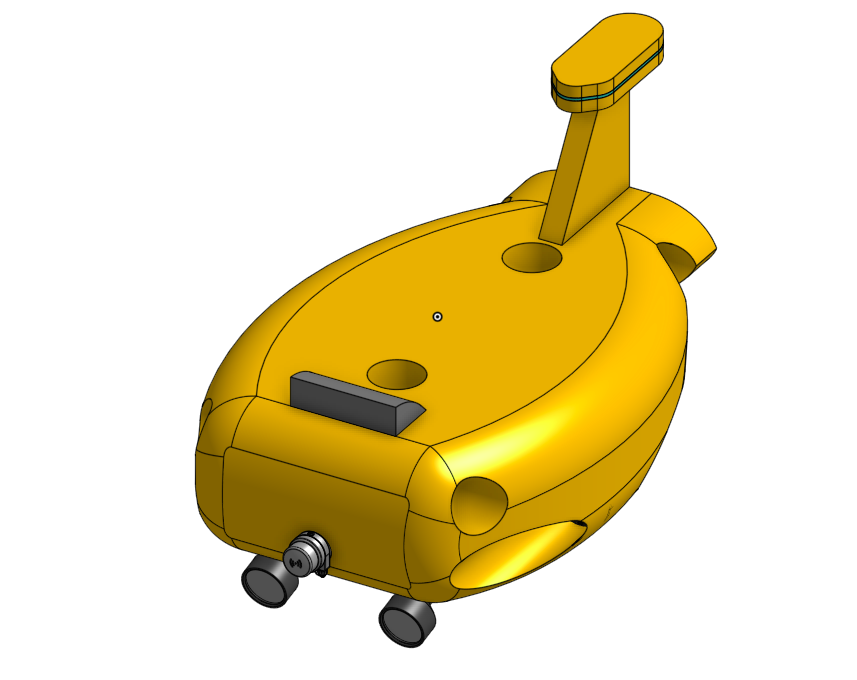
\includegraphics[height = 2.5cm, width=0.3\textwidth]{turbot-fish-01modi.png}
    
    \end{figure}
   
    
%*----------- notes
    \note[item]{Notes can help you to remember important information. Turn on the notes option.}
\end{frame}
%-
%*----------- SLIDE -------------------------------------------------------------
\begin{frame}[c]{Objetivo} 
    \transdissolve[duration=0.5]
   
    \begin{center}
        \Wider{%
        \begin{shaded}
        \begin{center}
            \vspace*{0.4cm}
            \resizebox{!}{1.3cm}{%
               % \color{bg} O objetivo é ter um objetivo.
                \begin{tabular}{ccc}
                    Desenvolver pesquisadores \\
                    na área de veiculos robóticos submarino
                     
                  \end{tabular}
            }%
        \end{center}
        \end{shaded}
        }%
    \end{center}
%*----------- notes
    \note[item]{Notes can help you to remember important information. Turn on the notes option.}
\end{frame}
%-
%*----------- SLIDE -------------------------------------------------------------
\begin{frame}[c]{Equipe}
    Os atuais membros da linha de pesquisa são

    \vspace*{1cm}

    \begin{center}
        \begin{figure}
            %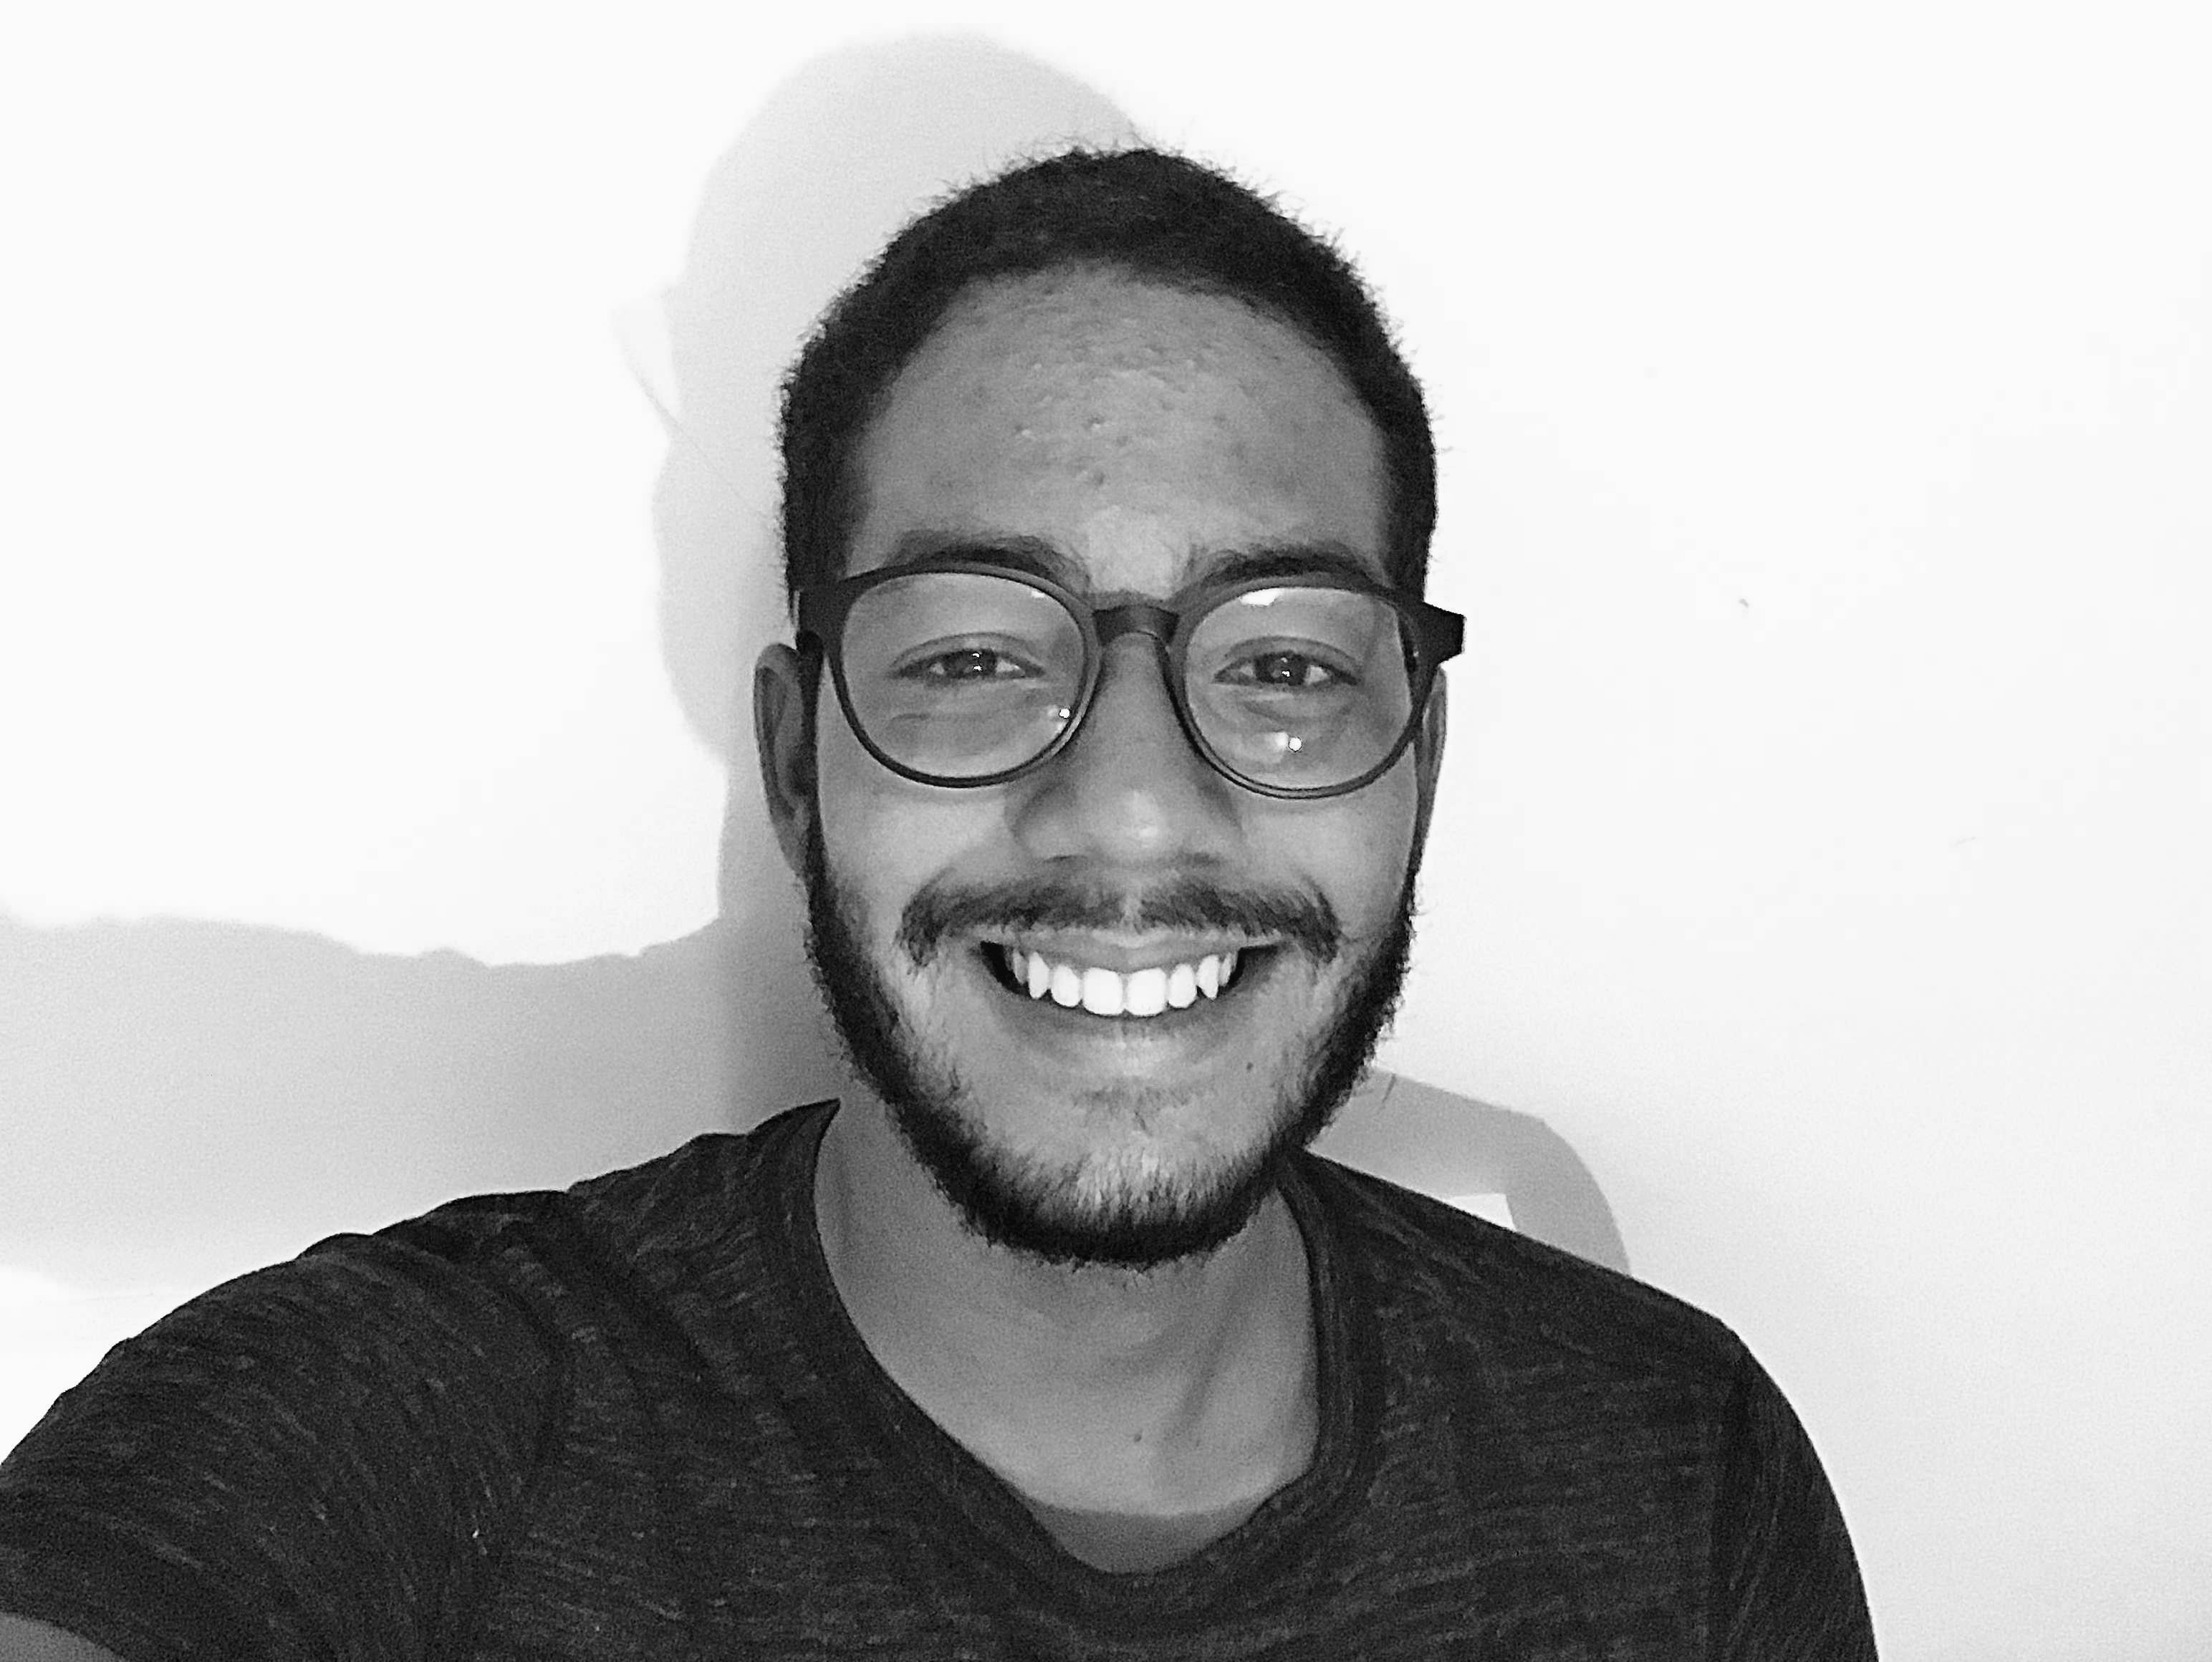
\includegraphics[width=0.45\textwidth]{alexandre.png}
            \roundpic[xshift=0cm,yshift=0cm]{1.915cm}{2.5cm}{alexandre}
            \caption{Alexandre Adonai}
        \end{figure}
         
            \begin{figure}
                
                \roundpic[xshift=0cm,yshift=0cm]{2.0cm}{2.5cm}{matheus1}
                \caption{Matheus Anselmo}
            \end{figure}    
          
            
     \end{center}
   
    
%*----------- notes
    \note[item]{Notes can help you to remember important information. Turn on the notes option.}
\end{frame}
%-

